\section{I курс}

\AddProb Однородный стержень массой $m$ и длиной $L$ вращают в горизонтальной плоскости с угловой скоростью $\omega$ вокруг одного из его концов. 
Найдите зависимость натяжения стержня от расстояния $x$ до оси вращении, если на другом конце закреплен маленький грузик массой $M$.

\AddProb Газовый термометр состоит из двух одинаковых сосудов  вместимости $V_0$ каждый, соединенных трубкой длины $L$ и сечения $S$. 
Трубку перекрывает капля ртути. Сосуды наполнены газом. Если температура газа в обоих сосудах одинакова, ртуть находится посередине трубки. 
Один сосуд помещен в термостат с температурой $T_0$. Проградуируйте термометр, находя зависимость температуры газа во втором сосуде 
от смещения ртути из положения равновесия.

\AddProb Однородный цилиндр радиуса $R$ и массы $m$ толкнули с начальной скоростью $v_0$ без вращения вдоль горизонтальной плоскости. 
Через какое время прекратится проскальзывание, если коэффициент трения цилиндра о плоскость равен $\mu$? Какая часть начальной энергии перейдет в тепло?


\section{II и III курсы}

\AddProb Газовый термометр состоит из двух одинаковых сосудов  вместимости $V_0$ каждый, соединенных трубкой длины $L$ и сечения $S$. 
Трубку перекрывает капля ртути. Сосуды наполнены газом. Если температура газа в обоих сосудах одинакова, ртуть находится посередине трубки. 
Один сосуд помещен в термостат с температурой $T_0$. Проградуируйте термометр, найдя зависимость температуры газа во втором сосуде 
от смещения ртути из положения равновесия.

% Почти задача (185) Колебания
\AddProb Проволочная вешалка качается с малой амплитудой в плоскости чертежа относительно заданных положений равновесия. 
В положениях а и б длинная сторона вешалки расположена горизонтально. Две другие стороны равны между собой. 
Во всех трех случаях (а, б, в) возникают колебания с одинаковыми периодами. Где расположен центр масс вешалки, если распределение массы в деталях неизвестно?

\begin{figure}[!h]
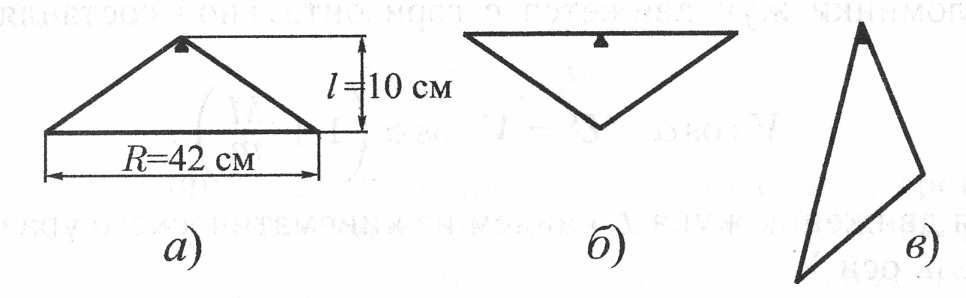
\includegraphics[scale=0.35]{1315OscillationsHanger.jpg}
\end{figure}

\AddProb Грани правильного додекаэдра равномерно заряжены с одинаковой поверхностной плотностью $\sigma$. 
В центре додэкаэдра помещен точечный заряд $ $. Определить силу, с которой точечный заряд действует на одну грань. Взаимодействие граней не учитывать. 